\documentclass[11pt, a4paper]{article}  %(或book)
%\documentclass{emulateapj}
%\usepackage[Lenny]{fncychap}  %(章节的格式设置)
\usepackage{titlesec}
\titleformat{\section}{\Large\bfseries}{\thesection}{1em}{}
\titleformat{\subsection}{\large\bfseries}{\thesubsection}{1em}{}
% \titleformat{\section}{标题的格式,包括字体,字体大小,加粗}{标题序号,\thesection是数字,可自定义如“Di \thesection Zhang”}{标题序号与标题文字之间空格的大小,用pt或em,不能省}{标题文字大小,用\large等,可缺省}
\usepackage{amsmath}
\usepackage{amssymb}
\usepackage{float}
\usepackage{natbib}
\usepackage{color}
\usepackage{mathrsfs}
\usepackage{graphicx}
\usepackage{CJK}  %(CJK宏包,也可以写成\usepackage{CJKutf8})
\usepackage{setspace}
\usepackage{graphicx}
\usepackage{multirow}
\usepackage{tabularx}
\usepackage{indentfirst} % indent at each head of graphy
\usepackage{subfigure} % 在\begin{figure}环境下插入横排并列的子图
\usepackage{multicol} % 部分页面的文字分栏设置(不适用于图片和表格)
\usepackage[top=3cm, bottom=3cm, left=2cm, right=2cm]{geometry}  %(边距)
% \newgeometry{left=..} % 会另起一新页,然后从该新页开始使用新的边距,直到遇到 \restoregeometry 为止

\begin{document}
\begin{CJK}{UTF8}{gbsn}  %(用UTF8编码,否则可能乱码,一定要3个{}都有)
\nocite{*}
\setlength{\parskip}{6pt}  % 设置标题上下的间距(\setlenght要在\begin{document}之后才有效果)
\setlength{\baselineskip}{20pt} % 设置每一行的行距

%\begin{figure}[htbp]/[H]
%%\center
%\includegraphics[width=xxcm]{figure.eps}
%\subfigure{ \includegraphics[width=xxcm]{test1.eps} } % 注意\subfigure后有{}
%\subfigure{ \includegraphics[width=xxcm]{test2.eps} } % 插入横排并列图片
%\subfigure{ \includegraphics[width=xxcm]{test3.eps} }
%\caption{Explain of figure}
%\label{fig:figurelabel}
%\end{figure}

%\begin{table}[htbp]/[H]
%\center
%\begin{tabular}{llcccr}  % number of columns, c->center, l->left, r->right
%\hline\hline  % \hline->horizontal line
%& Mass($M_{\text{sun}}$) & Radius(km) \\  % use "&" to align, "$$" to insert formula, "\\" to break the row
%\label{tab:tablelabel}
%\end{tabular}
%\end{table}

%\begin{eqnarray}
%	f(t) = \left\{ \begin{aligned}
%			a+bt & \, \quad t<0 \\
%			0    & \, \quad t \ge 0
%\end{aligned} \right.
%\end{eqnarray}


\title{\huge 直角坐标旋转和uvw坐标 \bf }

\author{Qizhi Huang}
\date{\today}
\maketitle
%%%%%%%%%%%%%%% Begin %%%%%%%%%%%%%%%


使用右手螺旋定则:

\indent\indent右手拇指指向被绕轴的正方向,剩下四指向手心旋转的方向为旋转角的正方向。 

转动矩阵:
\begin{equation}
	\text{新坐标} = \text{转动矩阵}R \cdot \text{旧坐标}
\end{equation} 

P点在直角坐标系$xyz$中的坐标为$(x,y,z)$。 

P点不动,直角坐标系$xyz$绕x轴转动$\alpha$角,变成新坐标系$xy'z'$,P点在新坐标系中的坐标为$(xy{'}z{'})$,有转动矩阵:
\begin{equation}
\begin{bmatrix} x \\ y' \\ z' \end{bmatrix} = R_x^c \begin{bmatrix} x \\ y \\ z \end{bmatrix} \qquad \Rightarrow \qquad R_x^c = \begin{bmatrix} 1 & 0 & 0 \\ 0 & \cos\alpha & \sin\alpha \\ 0 & -\sin\alpha & \cos\alpha \end{bmatrix}
\end{equation} 

P点不动,直角坐标系$xyz$绕y轴转动$\alpha$角,变成新坐标系$x'yz'$,P点在新坐标系中的坐标为$(x'yz')$,有转动矩阵:
\begin{equation}
R_y^c = \begin{bmatrix} \cos\alpha & 0 & -\sin\alpha \\ 0 & 1 & 0 \\ \sin\alpha & 0 & \cos\alpha \end{bmatrix}
\end{equation} 

P点不动,直角坐标系$xyz$绕z轴转动$\alpha$角,变成新坐标系$x'y'z$,P点在新坐标系中的坐标为$(x'y'z)$,有转动矩阵:
\begin{equation}
R_z^c = \begin{bmatrix} \cos\alpha & \sin\alpha & 0 \\ -\sin\alpha & \cos\alpha & 0 \\ 0 & 0 & 1 \end{bmatrix}
\end{equation} 


如果直角坐标系$xyz$不动,P点分别绕$x$轴、$y$轴、$z$轴转$\alpha$角得到新点P',求P'在$xyz$的坐标,可认为是P点不动,反方向旋转坐标系$-\alpha$角。P'的旋转矩阵为
\begin{equation}
	R_x^p = \begin{bmatrix} 1 & 0 & 0 \\ 0 & \cos\alpha & -\sin\alpha \\ 0 & \sin\alpha & \cos\alpha \end{bmatrix} \qquad 
	R_y^p = \begin{bmatrix} \cos\alpha & 0 & \sin\alpha \\ 0 & 1 & 0 \\ -\sin\alpha & 0 & \cos\alpha \end{bmatrix} \qquad
	R_z^p = \begin{bmatrix} \cos\alpha & -\sin\alpha & 0 \\ \sin\alpha & \cos\alpha & 0 \\ 0 & 0 & 1 \end{bmatrix}
\end{equation} 


\begin{figure}
\center
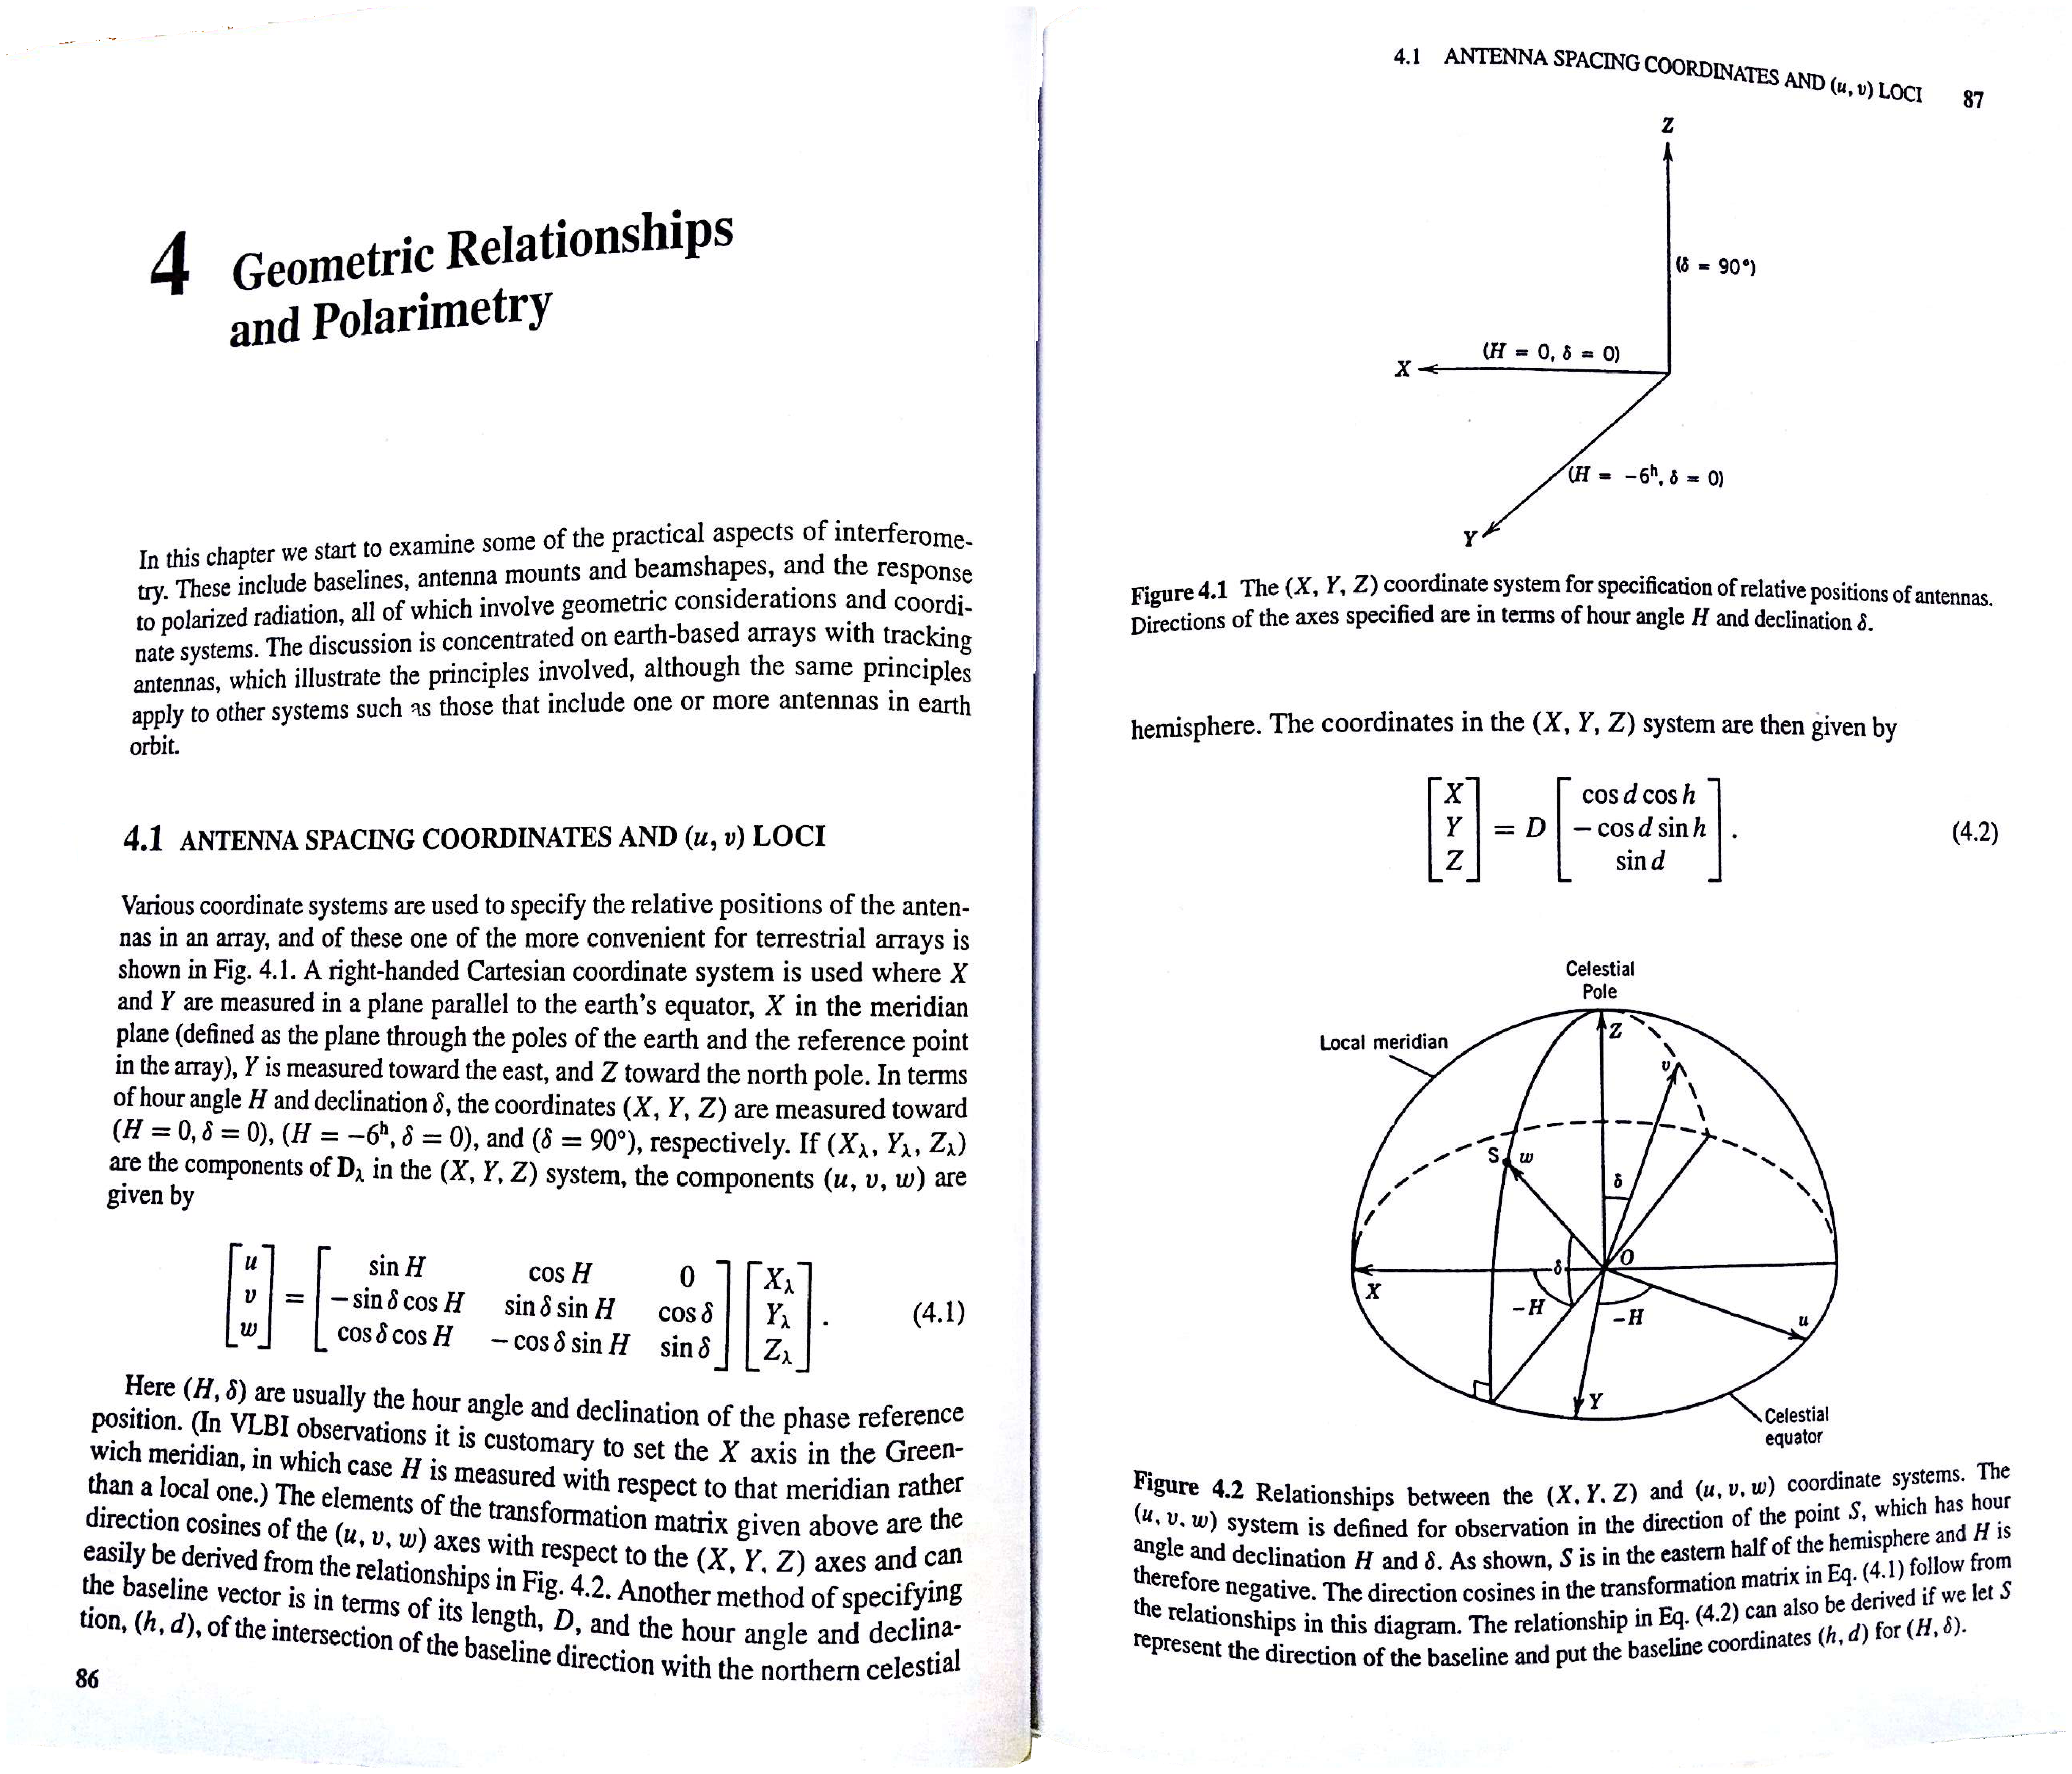
\includegraphics[width=16cm]{uvw_coordinate.eps}
\end{figure}



%%%%%%%%%%%%%%% End %%%%%%%%%%%%%%%
\end{CJK}
\end{document}
